\PassOptionsToPackage{unicode=true}{hyperref} % options for packages loaded elsewhere
\PassOptionsToPackage{hyphens}{url}
%
\documentclass[]{book}
\usepackage{lmodern}
\usepackage{amssymb,amsmath}
\usepackage{ifxetex,ifluatex}
\usepackage{fixltx2e} % provides \textsubscript
\ifnum 0\ifxetex 1\fi\ifluatex 1\fi=0 % if pdftex
  \usepackage[T1]{fontenc}
  \usepackage[utf8]{inputenc}
  \usepackage{textcomp} % provides euro and other symbols
\else % if luatex or xelatex
  \usepackage{unicode-math}
  \defaultfontfeatures{Ligatures=TeX,Scale=MatchLowercase}
\fi
% use upquote if available, for straight quotes in verbatim environments
\IfFileExists{upquote.sty}{\usepackage{upquote}}{}
% use microtype if available
\IfFileExists{microtype.sty}{%
\usepackage[]{microtype}
\UseMicrotypeSet[protrusion]{basicmath} % disable protrusion for tt fonts
}{}
\IfFileExists{parskip.sty}{%
\usepackage{parskip}
}{% else
\setlength{\parindent}{0pt}
\setlength{\parskip}{6pt plus 2pt minus 1pt}
}
\usepackage{hyperref}
\hypersetup{
            pdftitle={Perusall Quick-Start Guide},
            pdfborder={0 0 0},
            breaklinks=true}
\urlstyle{same}  % don't use monospace font for urls
\usepackage[margin=1.5in]{geometry}
\usepackage{longtable,booktabs}
% Fix footnotes in tables (requires footnote package)
\IfFileExists{footnote.sty}{\usepackage{footnote}\makesavenoteenv{longtable}}{}
\usepackage{graphicx,grffile}
\makeatletter
\def\maxwidth{\ifdim\Gin@nat@width>\linewidth\linewidth\else\Gin@nat@width\fi}
\def\maxheight{\ifdim\Gin@nat@height>\textheight\textheight\else\Gin@nat@height\fi}
\makeatother
% Scale images if necessary, so that they will not overflow the page
% margins by default, and it is still possible to overwrite the defaults
% using explicit options in \includegraphics[width, height, ...]{}
\setkeys{Gin}{width=\maxwidth,height=\maxheight,keepaspectratio}
\setlength{\emergencystretch}{3em}  % prevent overfull lines
\providecommand{\tightlist}{%
  \setlength{\itemsep}{0pt}\setlength{\parskip}{0pt}}
\setcounter{secnumdepth}{5}
% Redefines (sub)paragraphs to behave more like sections
\ifx\paragraph\undefined\else
\let\oldparagraph\paragraph
\renewcommand{\paragraph}[1]{\oldparagraph{#1}\mbox{}}
\fi
\ifx\subparagraph\undefined\else
\let\oldsubparagraph\subparagraph
\renewcommand{\subparagraph}[1]{\oldsubparagraph{#1}\mbox{}}
\fi

% set default figure placement to htbp
\makeatletter
\def\fps@figure{htbp}
\makeatother

\usepackage{booktabs}

\usepackage{epsfig}
\usepackage{epstopdf}
\usepackage{rotate}
\usepackage{graphicx}
\usepackage{hyperref}
\usepackage{alphalph}
\usepackage{caption}
\usepackage[hang,flushmargin]{footmisc}
\usepackage{framed}
\usepackage{xcolor}
\usepackage{verbatim} 

\usepackage{bm}
\setcounter{MaxMatrixCols}{20}
\newcommand{\Var}{\mathrm{Var}}
\newcommand{\SD}{\mathrm{SD}}
\newcommand{\Cov}{\mathrm{Cov}}
\newcommand{\fx}{f({\bf x})}
\newcommand\R{{\textsf R~}}
\newcommand\Rst{\textsf{RStudio}}

% spacing between environments
\usepackage{amsthm}
\makeatletter
\def\thm@space@setup{%
  \thm@preskip=15pt plus 2pt minus 4pt
  \thm@postskip=\thm@preskip
}
\makeatother


% Title format
\usepackage{titling}
\pretitle{\Huge\sffamily}
\posttitle{\par\vskip 0.5em}
\predate{\LARGE\sffamily}
\postdate{\par}

\urlstyle{tt}
\usepackage[]{natbib}
\bibliographystyle{apalike}

\title{Perusall Quick-Start Guide}
\author{}
\date{\vspace{-2.5em}January 2021}

\begin{document}
\maketitle

{
\setcounter{tocdepth}{1}
\tableofcontents
}
\hypertarget{what-is-perusall}{%
\chapter*{What is Perusall?}\label{what-is-perusall}}
\addcontentsline{toc}{chapter}{What is Perusall?}

\href{https://perusall.com/}{Perusal} is a browser-based software platform for interactive learning. Students help each other learn by collectively annotating readings in threads, responding to each other's comments, and interacting. Perusall can bring the interactivity of a small seminar to a larger course.

\hypertarget{why-are-we-using-perusall}{%
\section*{Why are we using Perusall?}\label{why-are-we-using-perusall}}
\addcontentsline{toc}{section}{Why are we using Perusall?}

Some of our Data Science Workshops are being taught using a ``flipped classroom'' model --- this is where lecture-based material is delivered online, asyncronously, so that it can be digested at your own pace, which provides more time for Q\&A discussion during in-class time.

Prior to our Zoom-based one-hour Q\&A session, there will be a \textbf{two week self-study period} during which you can work through the workshop materials at your own pace. We are using Persuall as a means to facilitate greater engagement with the workshop materials during this self-study period. With Perusall, you will be able to post questions and comments about parts of the materials you do not understand or problems you encounter. Instructors can answer your questions and comments, but you will also have the opportunity to reply to questions and comments from other participants. In this way, Perusall facilitates peer-to-peer and peer-to-instructor learning.

\textbf{Your successful completion of the workshop will be based on making a contribution, via questions and comments, during this self-study period.}

\hypertarget{how-to-use-perusall}{%
\chapter*{How to use Perusall?}\label{how-to-use-perusall}}
\addcontentsline{toc}{chapter}{How to use Perusall?}

You should have received an email asking you to create an account at \url{https://perusall.com/}. You should also have receive a \textbf{course code} via email. If you have not, please contact your workshop administrator. Once your Perusall account is created, enter the course code and you will be able to view the course materials.

During the two week self-study period, you can highlight sections of the workshop materials you wish to ask questions about, add comments, as well as respond to questions and comments from other participants. The window for submitting questions will close 24 hours prior to the Zoom Q\&A session.

\hypertarget{my-courses}{%
\section{My courses}\label{my-courses}}

\includegraphics{images/1_my_courses.png}

\hypertarget{get-started}{%
\section{Get started}\label{get-started}}

\includegraphics{images/2_get_started.png}

\hypertarget{assignments}{%
\section{Assignments}\label{assignments}}

\includegraphics{images/3_assignments.png}

\includegraphics{images/4_instructions.png}

\hypertarget{layout}{%
\section{Layout}\label{layout}}

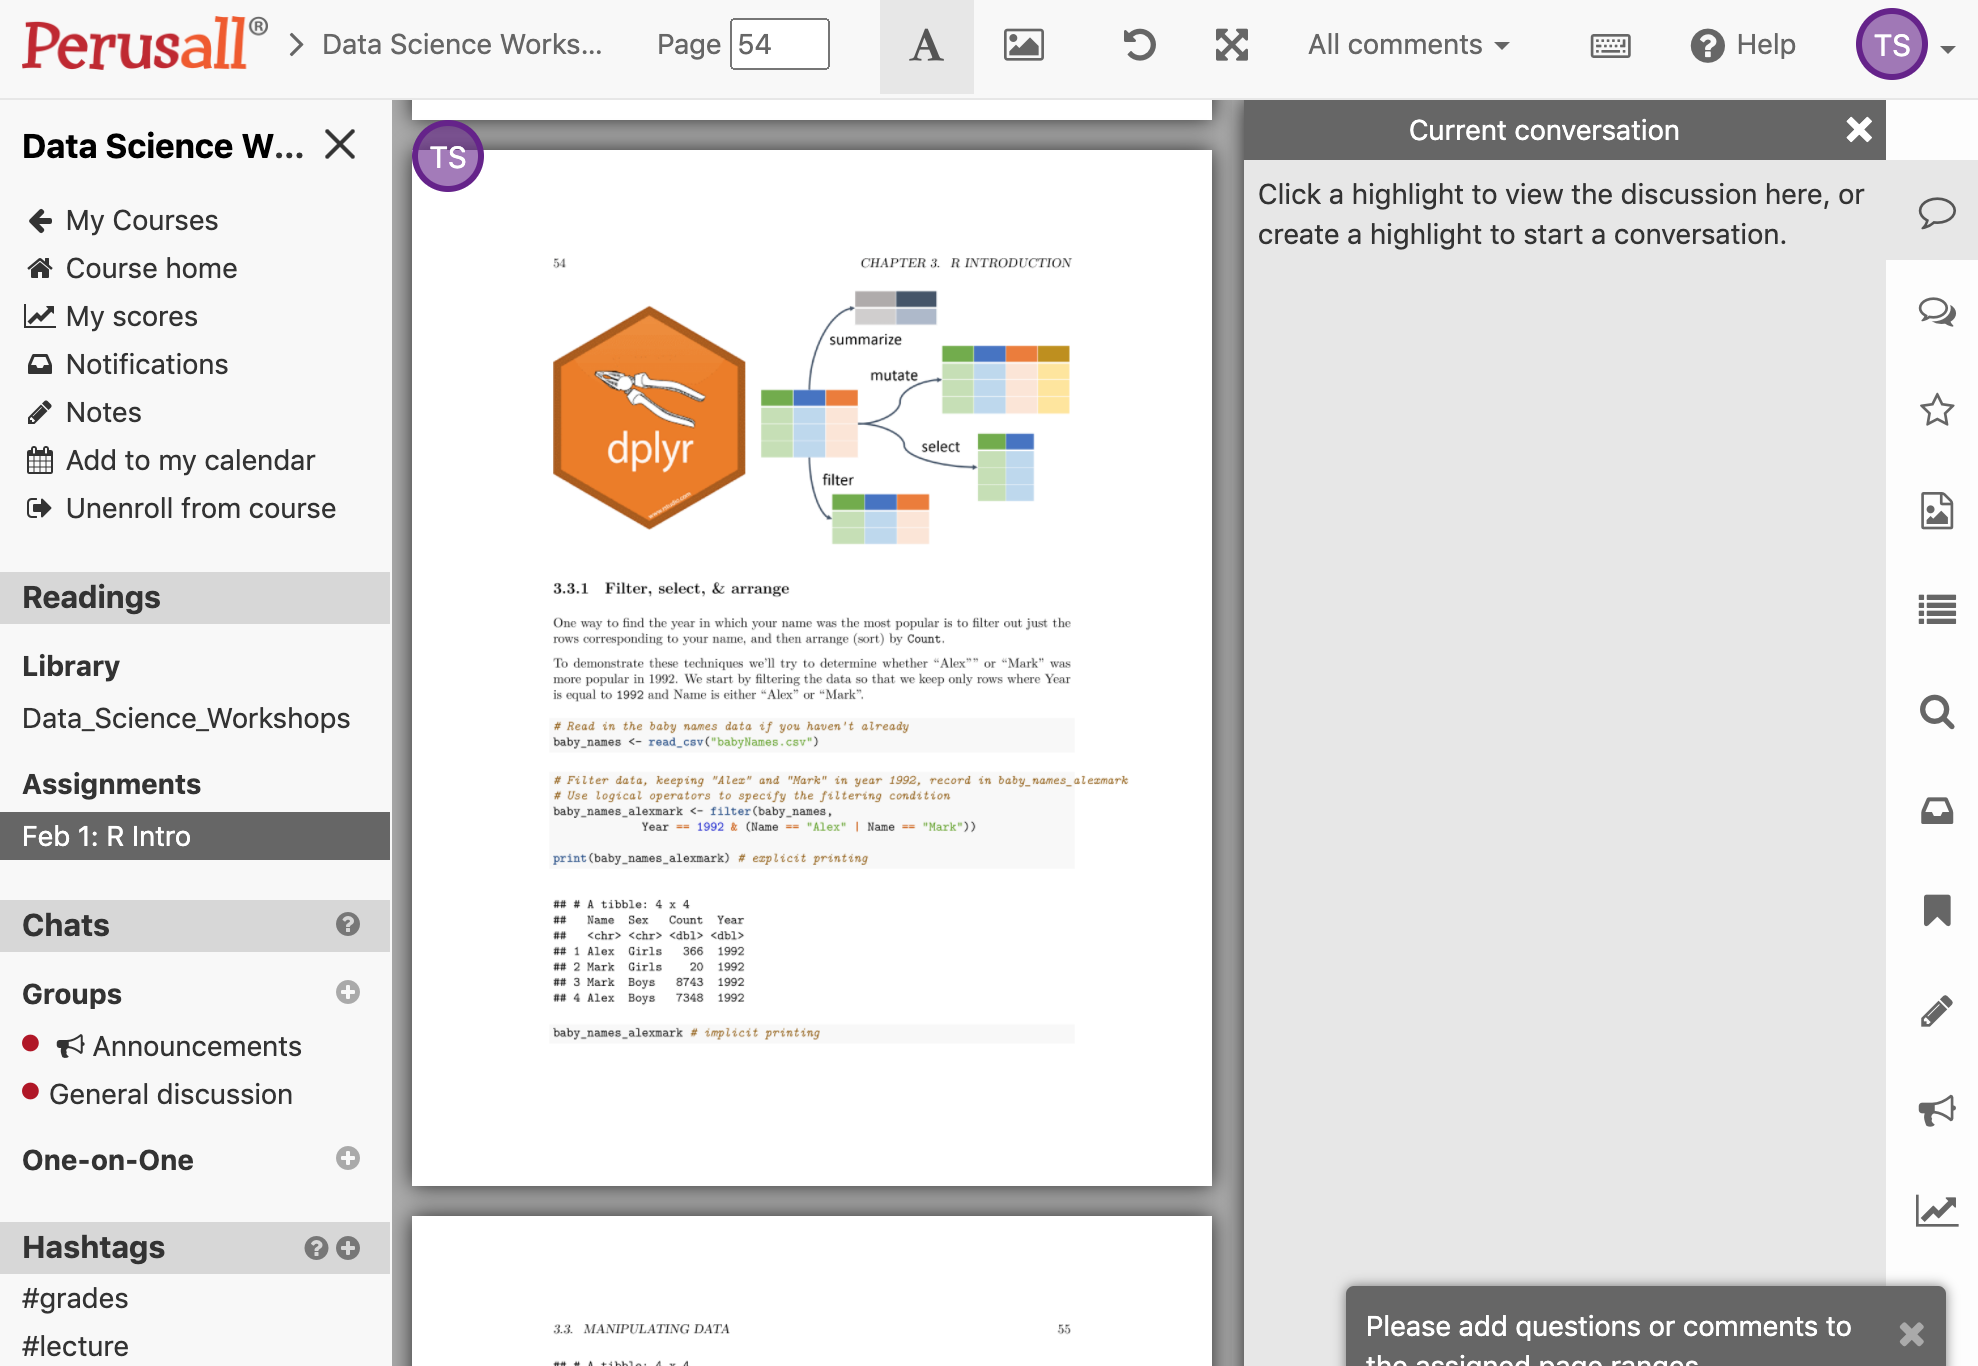
\includegraphics{images/5_layout.png}

\hypertarget{ask-a-question}{%
\section{Ask a question}\label{ask-a-question}}

\includegraphics{images/6_ask_question.png}

\hypertarget{answer-a-question}{%
\section{Answer a question}\label{answer-a-question}}

\includegraphics{images/7_answer_question.png}

\hypertarget{zoom-based-qa-session}{%
\chapter*{Zoom-based Q\&A session}\label{zoom-based-qa-session}}
\addcontentsline{toc}{chapter}{Zoom-based Q\&A session}

After the two-week self-study period, we will host a one-hour live Q\&A session via Zoom. No new material will be presented during this session -- rather, this will be an additional opportunity to ask questions and get feedback about the materials. The instructor will use the questions submitted on Perusall as a starting point for discussion and possibly for short code demonstrations illustrating conceptual or syntactical stumbling blocks.

\textbf{Zoom etiquette:} Pleasure be punctual. All participants will initially be entered into a Zoom waiting room and the presenter will admit them to the session at the designated start time. Any participants arriving in the wait room more than 5 mins past the listed start time of the session will not be admitted.

\end{document}
